\documentclass[10pt,twocolumn]{article}
\usepackage[letterpaper,margin=0.72in,columnsep=0.24in]{geometry}
\usepackage[T1]{fontenc}
\usepackage[utf8]{inputenc}
\usepackage{times}
\usepackage{microtype}
\usepackage{booktabs}
\usepackage{graphicx}
\usepackage{stfloats}
\usepackage[font=small,labelfont=bf,skip=3pt]{caption}
\usepackage[round]{natbib}
\setlength{\bibsep}{0pt}
\usepackage[most]{tcolorbox}
\usepackage[hidelinks]{hyperref}
\usepackage{titlesec}
\titlespacing*{\section}{0pt}{4pt}{1pt}
\titleformat{\section}{\normalsize\bfseries}{\thesection}{0.5em}{}
\setlength{\parskip}{1.5pt}
\setlength{\parindent}{0pt}
\raggedbottom
\setlength{\textfloatsep}{6pt}
\setlength{\dbltextfloatsep}{6pt}
\newtcolorbox{hypbox}{colback=gray!8,colframe=gray!60,boxrule=0.4pt,arc=1pt,left=3pt,right=3pt,top=2pt,bottom=2pt}
\newcommand{\XX}[1]{\textcolor{red}{#1}}

\title{\vspace{-0.62in}\large\textbf{Leaving for Europe, or Leaving Science?}\\[2pt]\normalsize Reading Parental Leave Policies at Scale to Explain Who Stays in US Academia}
\author{\normalsize Antoni Czolgowski \quad CSCI 7000 NLP for Cultural Analytics, Proposal 3, 27 October 2026}
\date{\vspace{-0.32in}}

\begin{document}
\maketitle

\section{Motivation and research questions}
Take two assistant professors hired in the same year, one at the University of Kentucky and one at the University of Nottingham, two universities of about the same size and the same mix of fields. Both have their first child. In Nottingham the policy gives her 26 weeks off at full pay. In Lexington she is paid while she recovers, ``usually 6--8 weeks'', under the faculty rules for temporary disability, and a colleague whose partner gives birth finds no paid leave in those rules at all. At CU Boulder either parent gets 18 weeks at full pay. In the US every university writes these rules for itself, while in most of Europe the state writes them and universities add something on top, or nothing.

I read these documents as culture written down. Besides the number of weeks, they say whom the institution imagines as the parent: a mother who has to recover, any parent who needs time with the child, or a ``primary caregiver'' who has to declare it. Kentucky's faculty rules treat a birth as a medical event, and Michigan's tenure-clock rule for childbearing is written for ``a woman who bears one or more children''. The wording is not neutral in its effects either. When top economics departments made tenure-clock extensions gender-neutral, men's tenure rates went up and women's went down \citep{antecol2018}.

Do these rules change who stays in science? Parenthood explains most of the gender gap in faculty productivity, and women, far more than men, say the leave policy mattered when they chose their job (45.9\% against 20.6\%, \citealp{morgan2021}). But a survey of current faculty only hears from the people who stayed. Following everyone in a census of 245,270 US faculty, \citet{spoon2023} show that women leave at higher rates at every career age, more often because of workplace climate than because of work-life balance. What this attrition cannot tell is where people went. A woman who takes a faculty job in Leuven and a woman who leaves research both disappear from the US census in the same way. The policy story makes a prediction about that destination. If more generous leave abroad pulls women out, their extra departures around the first birth should go to Europe. If family ties hold them in place, the extra departures should go out of science.

To test this I need the policies themselves, for hundreds of universities, on two continents, and for every year a career passes through, and this is where the question becomes a language problem. A leave policy is not a number in a table. It is a set of documents written by HR offices, faculty senates and unions, in different languages and legal traditions, and the number has to be read out of sentences like ``120 hours of paid family leave'', ``a one semester paid leave of absence'' for the ``primary care giver'', ``26 weeks' leave on full pay (inclusive of any SMP)'' or ``Der bezahlte Urlaub beträgt zwei Wochen''. \citet{morgan2018} collected the policies of 205 US and Canadian universities in 2018, which was a one-time effort. I propose an NLP pipeline that does this reading at scale: find the documents, keep the passages about leave, extract a fixed set of fields with an LLM that has to quote its evidence, check the extraction against independent coders, and follow the fields across archived versions of the same page. The second half of the project links the extracted policies to where people go when they leave US academia.

\begin{hypbox}
\textbf{RQ1 (policies).} How generous are faculty parental leave policies at US universities compared with matched European universities, whom do they address (mothers, parents, or a primary caregiver), and how did both change since 2011?\\[2pt]
\textbf{H1 (destination).} Around the first birth, women's extra departures from US science, relative to men's, go to Europe rather than out of science. \emph{Disconfirmed if}, at career ages 6--11, the women-to-men ratio of yearly rates is above 1 for exits but not for moves to Europe (95\% CIs).\\[2pt]
\textbf{H2 (policy).} These extra departures are smaller where the university or the state pays at least one semester of leave. \emph{Disconfirmed if} the gender $\times$ birth window $\times$ policy term of the hazard model in Section~7 has a 95\% CI that includes 0.
\end{hypbox}

\begin{figure*}[t]\centering
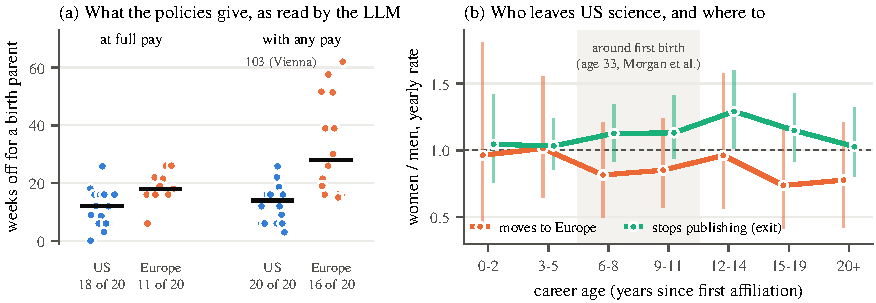
\includegraphics[width=\textwidth]{fig1.pdf}
\caption{(a) Weeks off for a birth parent at 20 US universities and their 20 European twins, as extracted by the LLM, at full pay and with any pay (bars are medians, ``$n$ of 20'' counts the texts that state the number). (b) Women-to-men ratio of yearly rates of leaving US science by career age, for moves to Europe and for exits, with 95\% CIs from 300 bootstrap resamples of authors. Shaded: the career ages where a first birth at the average faculty age of 33 \citep{morgan2021} most likely falls, if careers start in the mid-twenties.}
\end{figure*}

\section{Data}
\textbf{What I used in this pilot.} \emph{Policy documents.} I drew 20 US universities at random from the 80 most productive in OpenAlex \citep{priem2022}, 10 in states with a state paid family leave insurance program and 10 in states without one, with CU Boulder fixed in. For each I found a European \emph{twin}: the university closest in its share of output across 26 research fields, its number of works and its citations per work, matched one-to-one with an optimal assignment and at most four twins per country (11 countries, the UK, Switzerland and Poland allowed). The official pages were found with LLM-assisted web search restricted to university and government domains, and then downloaded by a script: faculty handbooks, HR and provost pages, union contracts, and for Europe the national government page when the university page referred to it. In total 92 documents, 551,000 words, in eight languages. \emph{The Wayback Machine} I used only in two small ways: to recover pages that blocked automated download, and to count how many archived versions six US policy pages have. \emph{Careers.} OpenAlex author records with yearly affiliations: three random samples of 10,000 authors ever affiliated with a US institution (10 to 1,000 works), and one sample of 10,000 authors ever in the US whose last affiliation is in Europe, to have enough movers.

\textbf{What the full study adds.} The AARC faculty census used by \citet{spoon2023}, licensed to a CU research group I now work with, gives who left a US faculty job and when, 2011 onwards, with field, rank and institution. OpenAlex then gives where each person went. The 2018 collection of 205 universities \citep{morgan2018} is the ground truth for validating the extraction on US policies, and the EPLP dataset \citep{spitzer2026} gives the national layer for Europe: maternity, co-parent and parental leave entitlements for 21 countries from 1970 to 2024. The Wayback Machine then becomes a real source: every archived version of every policy page since 2011.

\emph{Permissions.} The policies are public documents, fetched at a polite rate and not redistributed (the repository has the code to fetch them again). OpenAlex is CC0, and the Wayback Machine is open for research. AARC is licensed, so it would only be used with the agreement of the group that holds it, and linking census records to OpenAlex person by person is human-subjects data that needs IRB review. All results are reported in aggregate.

\section{Language features (operationalization)}
The NLP part is a pipeline of five steps, and each one is a place where the measurement can fail. (1) \emph{Retrieval}: an LLM agent with web search finds the official policy pages of a university, and a script downloads them, with the Wayback Machine as a fallback. (2) \emph{Passage selection}: union contracts and handbooks run to 50,000--80,000 words, so I cut every document into 120-word windows and keep the windows that mention leave in any of the eight languages (parental, maternity, childbirth, tenure clock, Mutterschutz, Elternzeit, congé maternité, föräldraledighet, and others), with their neighbors. (3) \emph{Extraction}: the LLM reads the passages for one reference person, a tenure-track assistant professor with two years of service and a first child, and fills a codebook of ten fields: weeks off at full pay for the birth parent and for the non-birth parent, weeks with any pay, semesters of teaching relief on top of the leave, the tenure clock (automatic, on request, none), a primary-caregiver clause, who pays, the service needed to qualify, whether the text relies on rules it does not state, and the framing. It converts units (a semester is 16 weeks, a quarter 11, 40 hours one week), and for every field it has to give a verbatim quote of at most 25 words and a confidence. A script checks that each quote really appears in the document. (4) \emph{Framing}: whether the rules are organized around the mother (maternity, paternity, a woman who bears a child), around the parent (parent, birth parent, caregiver), or both. (5) \emph{Versions}: the same extraction run on every archived version of a page, so a change in a field dates a change in the policy.

Why these features. The weeks and the teaching relief are what faculty mean when they say a policy mattered to them \citep{morgan2021}, and they are what a woman deciding between two offers would compare. The framing carries the cultural part of the question, whom the institution expects to do the caring, and it matters because rules that look neutral can still favor one parent \citep{antecol2018}. I compare fields across versions, not the pages, because the page around a policy changes much more often than the policy: the NYU handbook page has 31 different page hashes in 33 archived captures. And a keyword count cannot do this job, because the weeks hide behind unit conversions, caps (``up to''), conditions (``if the primary caregiver''), and references to national law.

\section{Feasibility test}
\textbf{Finding the documents: easy in the US, hard in Europe.} The matching paired all 20 universities, with one weak pair: Michigan has no European university of its size. I found official rules for all 20 US universities. Nine US pages refused automated download, and the Wayback Machine returned seven of them. In Europe it was different. Four of the 20 twins (Montpellier, Florence, Aix-Marseille, Copenhagen) have no public page on staff leave at all, because the rules sit on intranets behind a staff login, and several more publish only a summary. There, the public text is a sector collective agreement, like the Dutch universities' CAO, or the national law itself.

\textbf{Extracting and checking.} Claude Opus 5.5 extracted the codebook for all 40 universities. On a first pass it reported that Michigan's text was garbled and that Duke's and Case Western's leave sections had been cut off, and both were true: the Wayback copies of Michigan's pages were saved compressed, and my first passage selection kept whole paragraphs and lost the leave sections of the longest handbooks. After I fixed both, every quote passed the script check. As stand-ins for human coders, two models from other companies, GPT-6.1 Terra and Grok 4.7 Fast, coded 10 of the universities blind, from the same texts and with the same rules written as instructions for a human coder. Claude agrees with GPT on 51 and with Grok on 50 of the 60 cells, and with at least one of them on 58. All three agree on 9 of 10 birth-parent weeks but only on 5 of 10 framings. The disagreements are about the codebook, not about reading. Does a rule that is not stated mean zero weeks or a missing value? Where does ``mixed'' framing end and ``gendered'' begin? Is the UK rule that a mother must end her maternity leave before her partner can share it a primary-caregiver clause? These questions go into the codebook before the full run.

\textbf{What the policies say.} Where the text states it (Figure~1a), a birth parent gets a median of 12 weeks at full pay at the US universities and 18 at their European twins, higher in Europe in 7 of the 9 pairs where both numbers are stated, and 14 against 28 weeks with any pay. But the European number can be read from the documents for only 11 of the 20 twins, because the rest point to national law without stating it, so the full pipeline has to join the national layer from EPLP. The framing splits by continent. 17 of the 20 US texts speak only of parents, while 18 of the 20 European texts are built around maternity, alone (8) or next to parental terms (10). The change over time is recoverable: the University of California's policy alone has 9 distinct archived versions since 2014.

\textbf{Careers (H1): the first numbers lean against the pull story.} From the random samples, I kept authors whose careers began between 1990 and 2018 and whose first name could be gendered with a name dictionary \citep{genderguesser}, which is binary and failed on 37.5\% of names: 8,943 authors (3,651 women), observed in the US between 2000 and 2020. Career age is years since the first affiliation. A \emph{move to Europe} is a last US year followed by at least two years at a European institution, and an \emph{exit} is a last US year with no affiliation anywhere in the five or more years after. Women do not move to Europe more than men at any career age (Figure~1b, 0.81 [0.50, 1.21] at career ages 6--8), but they stop publishing more often than men, most clearly at 12--14 (1.29 [1.01, 1.60]). The counts are small (201 moves to Europe by women), names are a weak proxy, and stopping publishing is not the same as leaving academia, so this motivates the full test more than it answers it. One more fact already shapes the design: of 1,699 US-to-Europe movers in the second sample, 65\% began their careers in Europe, so most moves are returns home, and the model has to separate those who return from those who leave.

\section{Relation to existing work}
Leave policies have been collected for 205 US and Canadian universities \citep{morgan2018} and coded for the top economics departments \citep{antecol2018}, and for Europe they exist at the level of countries, not universities \citep{spitzer2026}. Work on faculty careers measures the productivity cost of parenthood \citep{morgan2021}, attrition and its reasons \citep{spoon2023}, and the prestige hierarchy that shapes hiring and moves \citep{wapman2022}, and work on the migration of scholars finds women less internationally mobile than men \citep{zhao2023}. None of it links careers to the text of the rules people lived under. On the NLP side, LLM coding matches trained annotators on some tasks and fails on others \citep{bamman2024,than2025}, which is why the extraction is checked by other coders, and \citet{gligoric2025} show how to draw valid conclusions from LLM labels when they are uncertain, which is how the extracted fields should enter the regressions. What I add is a panel of university leave policies read from text, on both continents and over time, and a link between it and where the people who leave actually go.

\section{Methods considered, and rejected}
\emph{Hand-coding everything}, as in 2018: about 400 PhD-granting US universities, their twins and 15 years of versions is too much reading, and it cannot be repeated every year. \emph{Keyword search for weeks} fails on hours, quarters and semesters, on ``up to'' caps and on who is eligible. \emph{One long prompt with all the policies}: given ten policies in one 30,000-word file, Grok reported four of them as missing, a small case of the long-context failures in \citet{karpinska2024}, so the pipeline reads one university at a time. \emph{Inferring births from paper acknowledgments or from gaps in publishing} is noisy and too private, so the timing of first births comes from the faculty survey of \citet{morgan2021}. \emph{Surveys of the people who left} are the best source for their reasons \citep{spoon2023}, and I keep them for a later stage.

\section{Limitations, ethics, next steps}
A policy on paper is not its use: 91.8\% of eligible mothers but 62.1\% of eligible fathers took leave \citep{morgan2021}, and departments negotiate their own arrangements. OpenAlex affiliations are noisy, and gender from names is binary and fails most on non-European names, which the full study replaces with the census's own gender records. The US funding cuts of 2025 and the European programs recruiting US scientists will confound the most recent years, so the main estimates stop before 2025. And the pilot shows associations only.

What I would do next, as the full study. (1) Collect the rules of every PhD-granting US university in AARC and of its European twin, every year from 2011, joined to the national layer. (2) Validate the extraction on the 2018 collection and on a random 10\% of policy versions double-coded by trained student coders or Prolific workers screened with a short quiz, use a panel of LLM coders from different companies to send their disagreements to humans, and carry the remaining error into the regressions \citep{gligoric2025}. (3) Link the people who leave AARC to their next affiliation in OpenAlex. (4) Fit a competing-risks model of each faculty-year, with five outcomes (stay, move within the US, move to Europe, move elsewhere, exit) and the gender $\times$ birth window $\times$ policy term of H2, separating returns home by the country of the first affiliation. For a causal estimate, the state paid leave programs started in different years, from California in 2004 to Colorado in 2024, and the Wayback Machine dates the changes in university policies, so the policy effect can be estimated as a staggered difference-in-differences. (5) From the model, calculate how many exits of women a one-semester floor would have prevented, and what those exits cost a university: a new faculty search, a new start-up package, and the research the person would have produced. (6) Write it up as a short brief for university leaders and state legislators.

\section*{Team}
Antoni Czolgowski (solo): question, design, data, experiments and writing.

\section*{Acknowledgments}
Readings that shaped the idea: \citet{gligoric2025}, \citet{bamman2024}, \citet{than2025} and \citet{karpinska2024}, which I presented in class as the archaeologist. AI use: Claude Opus 5.5 (in Claude, medium reasoning) helped me find the official policy pages, write the twin matching, collection and OpenAlex code, run the codebook extraction, make the figure and edit the text. GPT-6.1 Terra (ChatGPT, medium reasoning) and Grok 4.7 Fast were the second and third coders, run by me in fresh chats with the same rules. Code, codebook and extracted fields: \url{github.com/AntoniCzolgowski/parental-leave-nlp4ca}.

\small
\begin{thebibliography}{99}
\bibitem[Antecol et~al.(2018)]{antecol2018} H. Antecol, K. Bedard, J. Stearns. 2018. Equal but inequitable: Who benefits from gender-neutral tenure clock stopping policies? \emph{American Economic Review} 108(9):2420--2441.
\bibitem[Bamman et~al.(2024)]{bamman2024} D. Bamman, K. K. Chang, L. Lucy, N. Zhou. 2024. On classification with large language models in cultural analytics. \emph{Computational Humanities Research (CHR) 2024}, CEUR 3834.
\bibitem[Gligori\'c et~al.(2025)]{gligoric2025} K. Gligori\'c, T. Zrnic, C. Lee, E. Cand\`es, D. Jurafsky. 2025. Can unconfident LLM annotations be used for confident conclusions? \emph{NAACL 2025}.
\bibitem[gender-guesser(2016)]{genderguesser} gender-guesser. 2016. Python package, based on J. Michael's name dictionary. \url{pypi.org/project/gender-guesser}.
\bibitem[Karpinska et~al.(2024)]{karpinska2024} M. Karpinska, K. Thai, K. Lo, T. Goyal, M. Iyyer. 2024. One thousand and one pairs: A ``novel'' challenge for long-context language models. \emph{EMNLP 2024}.
\bibitem[Morgan et~al.(2018)]{morgan2018} A. C. Morgan, S. F. Way, M. Galesic, D. B. Larremore, A. Clauset. 2018. Paid parental leave at US and Canadian universities. Online dataset, CU Boulder and Santa Fe Institute.
\bibitem[Morgan et~al.(2021)]{morgan2021} A. C. Morgan, S. F. Way, M. J. D. Hoefer, D. B. Larremore, M. Galesic, A. Clauset. 2021. The unequal impact of parenthood in academia. \emph{Science Advances} 7(9):eabd1996.
\bibitem[Priem et~al.(2022)]{priem2022} J. Priem, H. Piwowar, R. Orr. 2022. OpenAlex: A fully-open index of scholarly works, authors, venues, institutions, and concepts. arXiv:2205.01833.
\bibitem[Spitzer et~al.(2026)]{spitzer2026} S. Spitzer, A. Lemoine, Z. Song, et al. 2026. The European Parenting Leave Policies (EPLP) dataset: Leave duration entitlements for 21 countries from 1970 to 2024. \emph{Demographic Research} 54(31):987--1008.
\bibitem[Spoon et~al.(2023)]{spoon2023} K. Spoon, N. LaBerge, K. H. Wapman, et al. 2023. Gender and retention patterns among U.S. faculty. \emph{Science Advances} 9(42):eadi2205.
\bibitem[Than et~al.(2025)]{than2025} N. Than, L. Fan, T. Law, L. K. Nelson, L. McCall. 2025. Updating ``the future of coding'': Qualitative coding with generative large language models. \emph{Sociological Methods \& Research} 54(3):849--888.
\bibitem[Wapman et~al.(2022)]{wapman2022} K. H. Wapman, S. Zhang, A. Clauset, D. B. Larremore. 2022. Quantifying hierarchy and dynamics in US faculty hiring and retention. \emph{Nature} 610:120--127.
\bibitem[Zhao et~al.(2023)]{zhao2023} X. Zhao, A. Akbaritabar, R. Kashyap, E. Zagheni. 2023. A gender perspective on the global migration of scholars. \emph{PNAS} 120(10):e2214664120.
\end{thebibliography}
\end{document}
